%- HandOut Flag -----------------------------------------------------------------------------------------
\newif\ifHandout
	\Handouttrue  %uncomment for the printable version

%- D0cum3nt ----------------------------------------------------------------------------------------------
\documentclass[beamer,10pt]{standalone}
	%\setbeameroption{show notes}
	




%- Packages ----------------------------------------------------------------------------------------------
%\usepackage{verbatim}
\usepackage[mode=buildnew,subpreambles=true]{standalone}
\usepackage{import}
\usepackage{amsmath, amssymb}
\usepackage{tikz}
%\usetikzlibrary{arrows,shapes,calc}
%\usetikzlibrary{shapes.callouts}
\usepackage{tikz-cd}
\usepackage{hyperref}
\usepackage[english]{babel}
\usepackage{stackengine}

%--Beamer Style-----------------------------------------------------------------------------------------------
\usetheme{toninus}



%--Beamer Style-----------------------------------------------------------------------------------------------
\usetheme{toninus}





%---------------------------------------------------------------------------------------------------------------------------------------------------
%- D0cum3nt ----------------------------------------------------------------------------------------------------------------------------------
\begin{document}
%------------------------------------------------------------------------------------------------

%##################################################################################
\section{Background Material}
%##################################################################################

%------------------------------------------------------------------------------------------------
\begin{frame}[fragile]{MS geometry and classical field mechanics}\label{Frame:Ms-Field-Mechanics}
		Consider a smooth manifold $Y$,
		\begin{columns}
			\hfill
			\begin{column}{.5\linewidth}
				\emph{Multicotangent bundle} $\bigwedge = \bigwedge^n T^\ast Y$\\
				is naturally $n$-plectic
			\end{column}
			\begin{column}{.4\linewidth}
				\[
				\begin{tikzcd}
					\Lambda \ar[d,"\pi"'] & T \Lambda \ar[d,"T \pi"] \ar[l] \\
					Y								& T Y \ar[l]
				\end{tikzcd}	
				\]
			\end{column}
		\end{columns}
	\pause
	\begin{defblock}[Tautological $n$-form]
		$\theta \in \Omega^n(\Lambda)$ such that:
		\begin{displaymath}
		\begin{split}
			\left[ \iota_{u_1 \wedge \ldots \wedge u_n} \theta \right]_\eta 
			&= \iota_{(T \pi)_\ast u_1 \wedge \ldots \wedge (T \pi)_\ast u_n} \eta \\
			&= \iota_{u_1 \wedge \ldots \wedge u_n} \pi^\ast \eta 
			\qquad \qquad \forall \eta \in \Lambda \, , \: \forall u_i \in T_\eta \Lambda 		
		\end{split}
		\end{displaymath}
	\end{defblock}
	\vfill
	\begin{columns}
		\begin{column}{.6\linewidth}
			\begin{defblock}[Tautological (multisymplectic) (n+1)-form]
				$$\omega := d \theta$$
			\end{defblock}
		\end{column}
		\begin{column}{.4\linewidth}
		 	\begin{claimblock}$\omega$ is not degenerate.\end{claimblock}	
		\end{column}
	\end{columns}	
	\pause
	\begin{keywordblock}
		\begin{tabular}{|c|c|c|}
			\hline 
			point-particles mechanics & $\rightsquigarrow$ & classical fields mechanics \\
			%(finite discrete DOF) & & (finite dimensional continuous DOF) \\
			\hline 
			symplectic & $\rightsquigarrow$ & multisymplectic \\ 
			\hline 
			Observables (Poisson) algebra & $\rightsquigarrow$ & Observables $L-\infty$ algebra
			 \\ 
			\hline 
			Co-moment map & $\rightsquigarrow$ & Homotopy co-momentum map \\ 
			\hline 
		\end{tabular} 
	\end{keywordblock}

	
\end{frame}
\note[itemize]{
	\item This example is significant from the perspective of geometric classical field theory:
		\begin{displaymath}
			\frac{\text{classical mechanics}}{\text{symplectic geo.}} =
			\frac{\text{classical field mechanics}}{\text{multisymplectic geo.}}
		\end{displaymath}
	\item Multicotangent bundle is the \emph{Higher analogue} of the cotangent bundle.
	(but it is not yet the analogue of a \emph{phase space}.)
\item The multiphase space is the sub-bundle of $n$-forms vanishing when contracted with 2 vertical fields.
  	\item The reason why this sub-bundle has a particular role is that it can be proved to be isomorphic to a suitable dual of the first Jet bundle.
  	\item For further details see Gotay et al. \href{https://arxiv.org/abs/physics/9801019}{arXiv:physics/9801019}. For a pictorial representation of all the structures involved in the geometric mechanics of I order classical field theories see appendix, pag: \ref{frame:Gimmsy}.
}
%------------------------------------------------------------------------------------------------	
	
%------------------------------------------------------------------------------------------------
\begin{frame}{Special classes of smooth objects}\label{Frame:Classes-Multisymplectic-Objects}
  	\begin{columns}
		\begin{column}[t]{.42\linewidth}		
			\begin{defblock}[Hamiltonian v.f.]
				$\mathfrak{X}_{ham} =  \left\lbrace X \in  \mathfrak{X} \right\vert \left. \iota_x \omega \textrm{ exact}  \right\rbrace$ 			
			\end{defblock}
			\begin{defblock}[Multisymplectic v.f.]
				$\mathfrak{X}_{ms} =  \left\lbrace X \in  \mathfrak{X} \right\vert \left. \mathcal{L}_X \omega = 0  \right\rbrace$ 	
			\end{defblock}
		\end{column}
		\begin{column}[t]{.58\linewidth}		
			\begin{defblock}[Hamiltonian $(n$-$1)-$forms]
				\begin{displaymath}
					\Omega^{n-1}_{ham} 	:=
					\biggr\{ H \in  \Omega^{n-1} \; \left\vert \; 
					\stackanchor{$\exists X \in \mathfrak{X}_{ham}$}{: $d H = -\iota_X \omega$} \right\} 
			\end{displaymath}
			\end{defblock}		
		\end{column}
  	\end{columns}
  	%
  	\vspace{0.5em}
  	%
  	\onslide<2->{
  	\begin{columns}
		\begin{column}[t]{.5\linewidth}	
			\centering\emph{Global symmetries}
			\begin{defblock}[Multisymplectic (Lie group) action]
				$\Phi: G \circlearrowright (M, \omega)$ \emph{right action} s.t. \\
				$$\hat{\Phi}(g)_\ast \omega = \omega \quad \forall g \in G$$
			\end{defblock}
		\end{column}
		\begin{column}[t]{.5\linewidth}			
			\centering\emph{Infinitesimal symmetries}
			\begin{defblock}[Multisymplectic (Lie algebra) action]
				$V: \mathfrak{g} \rightarrow \mathfrak{X} (M)$ \emph{Lie algebra morphism} s.t. \\
				$$\mathcal{L}_{V_\xi} \omega = 0 \quad \forall \xi \in \mathfrak{g}$$	
			\end{defblock}
		\end{column}
  	\end{columns}
  	}
  	%
  	\onslide<3->{		
	  	\begin{asideblock}[Hierarchy of conserved quantities]%Shades of...
	  		\begin{table}[] % http://tablesgenerator.com/
			\begin{tabular}{lllll}
					& strictly conserved & & & $\mathcal{L}_X \alpha= 0$ \\
				$\alpha \in \Omega^\bullet$ & globally conserved & along $X \in \mathfrak{X}$ & $\Leftrightarrow$ & $\mathcal{L}_X \alpha\in B $ (exact) \\
				  & locally conserved  & & & $\mathcal{L}_X \alpha\in Z $ (closed)                                
			\end{tabular}
			\end{table}
	  	\end{asideblock}
  	}
  	
  \end{frame}
  \note[itemize]{
  	\item Exactly as it happens in symplectic geometry, fixing a smooth form $\omega$ on $M$ yields a criterion for classifying vector fields and differential forms.
  	\\(Pay attention to the sign convention in defining the Hamiltonian vector fields)
  	\item Also, we can naturally select a special class of symmetries (global and infinitesimal) which preserve the fixed multisymplectic form.
  	\item Aside, we can start to see that, in this setting, measurable quantities are not only smooth functions but also differential forms with degree greater then zero.
  	For such objects can be defined weaker notions of conservation along a flow.
  	\item The idea to consider forms of various degree as observables do not fall out of the sky. 
  		For instance in a string there will be two kind of measurable quantities: extensive observable (1-forms), like the density, and intensive observables (0-forms), like the tension. 
 		%\href{https://en.wikipedia.org/wiki/Intensive_and_extensive_properties#Intensive_properties}{(wiki link on this terminology)}
  	\item Starting from this observation we can define the space of all possible observables (see next slide).
  }
%---------------------------------------------------------------------------------------------------------------------------------------------------

\begin{frame}[fragile,shrink]{Unwrapping the \emph{higher Jacobi equations}}\label{Frame:unwapping-Jacobi}
\underline{Slogan:} \emph{Jacobi identity satisfied up to an higher coherent homotopy}
		%
		\vspace{1.5em}
		\begin{columns}[c]
			\hfill
			\begin{column}{0.5\linewidth}
				Higher Jacobi implies:
				\begin{itemize}  \setlength\itemsep{1em}
					\item Underlying chain-complex $(L,\mu_1)$ with differential $d=\mu_1$;
					\item \color{red} $\mu_2 = [\cdot,\cdot]$ is a chain map $L^{\otimes 2} \to L$;
					\item \color{green!20!black}$\mu_3=j(\cdot,\cdot,\cdot)$ is a chain homotopy 
						$\mu_2\circ\mu_2 \Rightarrow 0$;
						\\ i.e. between the usual Jacobiator ${[[\cdot,\cdot],\cdot]} \circ P_{\text{unsh}}$ and the $0$ map 
					\item \color{purple}higher analogues...	
					\\ e.g. $\mu_4$, is a second order chain-homotopy between the two chain homotopies  ${[j(\cdot,\cdot ,\cdot]),\cdot]}\circ P_{\text{unsh}}$ and ${j([\cdot , \cdot],\cdot,\cdot)}\circ P_{\text{unsh}}$
				\end{itemize}
			\end{column}
			\begin{column}{0.45\linewidth}
				\includestandalone[width=0.9\linewidth]{Pictures/Figure_Linfinity_diagram}
			\end{column}	
		\end{columns}	
		\vspace{1.5em}
		Notation: $P_{\text{unsh}}$ = sum on all the possibile unshuffled permutation.

\end{frame}
\note[itemize]{
  \item Regarding any $l_k$ as a tree with $k$ entries and 1 output, the $k$-th generalized Jacobi equation is produced summing all the possible way to obtain a $k+1$-ary tree by composing two other trees (not more then two!).
  \item Can be regarded as
  	\begin{displaymath}
  		\sum_{i+j = k} l_j \circ ( l_j \otimes \mathbb{I}) \circ P_{\text{unsh}}
  	\end{displaymath}
  	Where $P_{\text{unsh}} : L^{\otimes(k-1)} \rightarrow L^{\otimes(k-1)} $ is the $(i,j)$-unshuffolator.
  	\\(you consider only unshuffles to avoid the redundancies given by the fact that any $l_i$ has fixed symmetry.
  \item Examples of unshuffles: \\
  \begin{displaymath}
  \begin{split}
  	(12)(3)\quad(13)(2)\quad(23)(1)\\
  	(123)(4)\quad(234)(1)\quad(134)(2)\quad(124)(3)\\
  	(12)(34)\quad(23)(14)\quad(13)(24)\quad(14)(23)\quad(24)(13)
  \end{split}
  \end{displaymath}
	\item When regarding the L$\infty$ structure as a chain complex with homotopies you get a neat intepretation of the Jacobi identity at the price that \emph{graded skew-symmetry} definition is more obscure than in the presentation with graded vector spaces.
}
%------------------------------------------------------------------------------------------------



%------------------------------------------------------------------------------------------------

% Frame inspired by Leonid: passing from moment maps to comoment maps
\begin{frame}[fragile]{Reminder: Moment maps in symplectic geometry}
	Let $(M,\omega)$ be a symplectic manifold, $\vartheta: G\times M \to M$ a Lie group action preserving $\omega$ and $v:\mathfrak{g}\to \mathfrak{X}(M)$ the corresponding infinitesimal action
	%
		\begin{defblock}[Moment map pertaining to $\vartheta$]
			Smooth map $ \mu: M \to \mathfrak{g}^\ast$ such that: \stackunder{$d \langle\mu , \xi \rangle = \iota_{v_\xi}\omega \scriptstyle\quad \forall \xi \in \mathfrak{g}$}{$f (\vartheta_g(x)) = Ad^\ast_g (f(x)) \scriptstyle\quad \forall g \in G, x \in M$}
		\end{defblock}
	%
	\vfill
	\emph{... from a dual perspective (assuming $G$ connected) ...}
			\begin{defblock}[Comoment map pertaining to $v$]
				\begin{columns}
					\begin{column}{.5\linewidth}	
			Lie algebra morphism \qquad $ f: \mathfrak{g} \to C^\infty(M) $
			\\
			such that \qquad $ d~f (x) = -\iota_{v_x} \omega \qquad \forall x \in \mathfrak{g}~.$
					\end{column}
					\begin{column}{.4\linewidth}	
						\begin{displaymath}
							\begin{tikzcd}
								& C^{\infty}(M,\omega) \ar[d]
								\\
								\mathfrak{g} \ar[ur,dashed,"(f)"]\ar[r,"v"']& \mathfrak{X}(M)
							\end{tikzcd}	
						\end{displaymath}
					\end{column}
				\end{columns}
		\end{defblock}		
	%
	\vfill
	\emph{... a tool encoding conserved quantities ...}
	\begin{propblock}[Noether Theorem]
		\small Fixed $H\in C^\infty_{\text{Ham}}(M)$ ($\mathfrak{g}$-invariant) ,
				$$\mathcal{L}_{v_H} f(x) = 0 \qquad \forall x \in \mathfrak{g}$$
	\end{propblock}
\end{frame}
%\note[itemize]{
%	\item comoment map is a Lie algebra morphism projecting to $v$. (Triangle diagram in Lie algebra category).
%}



%------------------------------------------------------------------------------------------------
\begin{frame}{Geometry of symmetries}\label{frame:geometrysymmetries}
	Basic mechanical structures are encoded in geometry. but there is another complementary geometrical property that's natural in physics: symmetry!
	\begin{alertblock}{Upshot}
		Continous symmetries are described by actions of a Lie group on $M$.
	\end{alertblock}
	\begin{block}{Noether}
		Presence of symmetries $\quad \Rightarrow \quad$ existence of conserved quantities.
	\end{block}	
	\begin{block}{Key concept:}
		Noether current are encoded in a \emph{moment map}  $\mu :M \rightarrow \mathfrak{g}^*$ (the dual of the comoment map $f$. 
	\end{block}
  \begin{columns}[T]
   	\begin{column}{.6\textwidth}
			\begin{block}{Symplectic reduction:}
			\begin{itemize}
				\item System dynamics should be restricted to level set of conserved observables in order to efficiently store dynamical properties.
				\item Under certain assumptions, $\mu^{-1}( 0 )/G$ is a symplectic manifold with an "induced" symplectic structure.
			\end{itemize}
			\end{block}
    \end{column}
    \begin{column}{.4\textwidth}	
			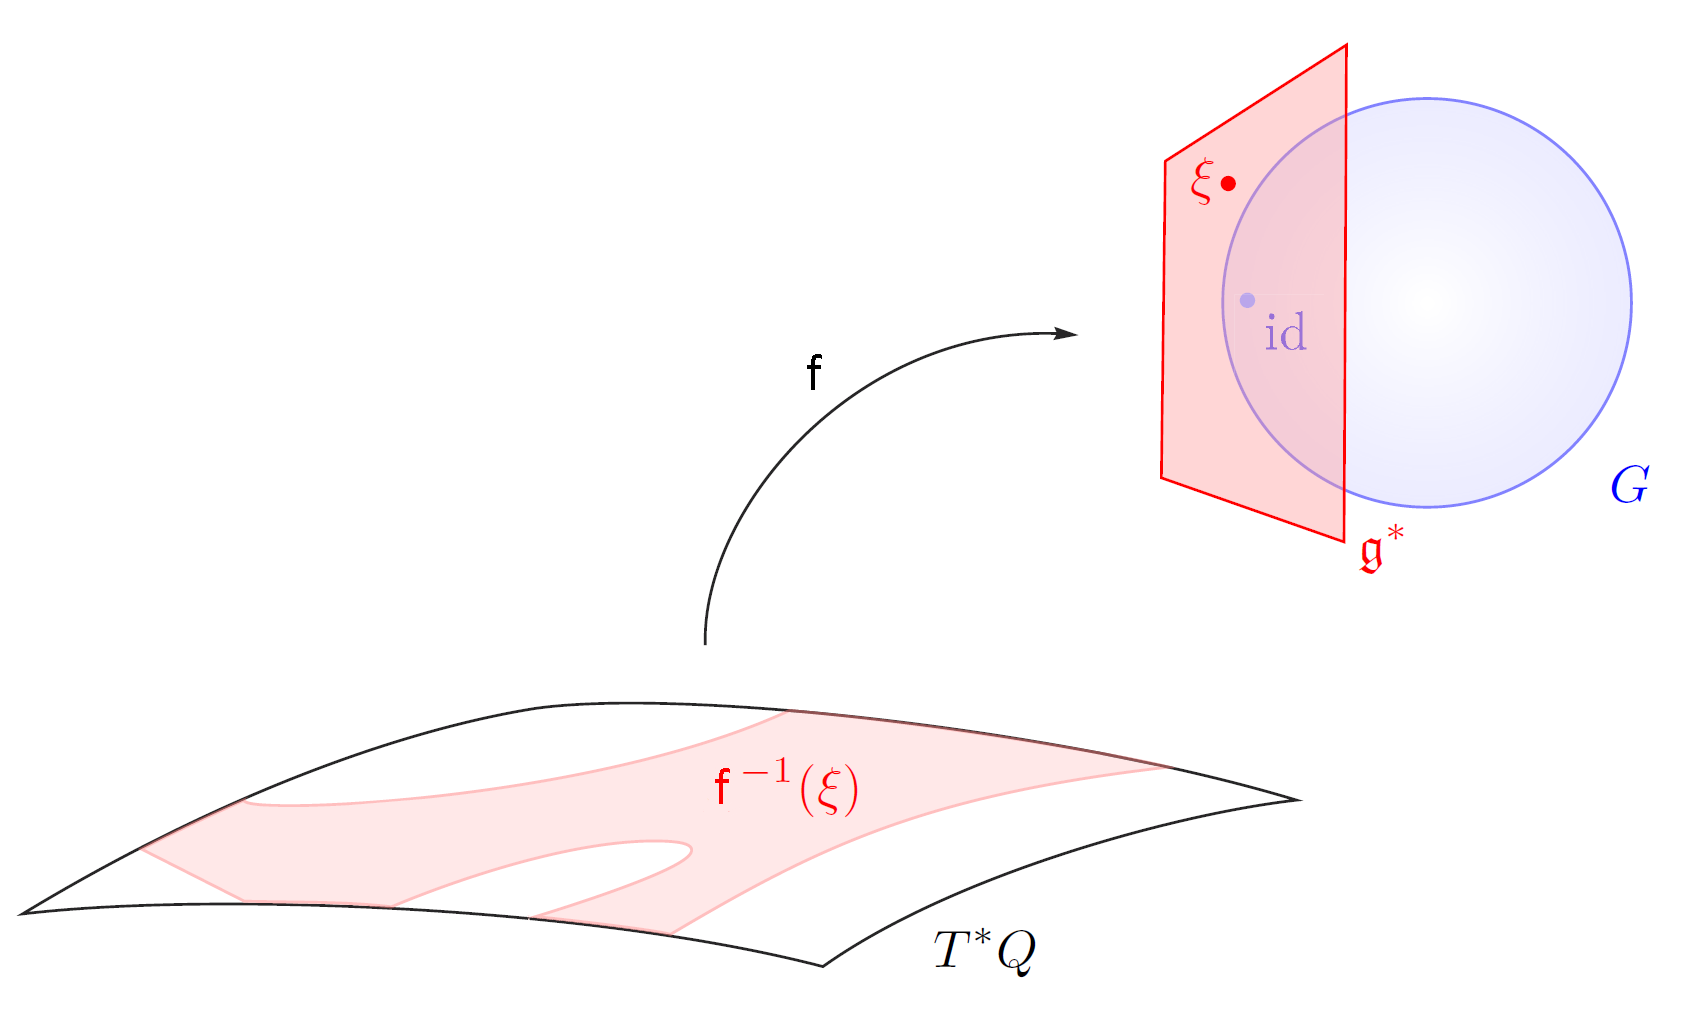
\includegraphics[width=\textwidth]{Pictures/Reduction} 
  	\end{column}
	\end{columns}			
\end{frame}
%------------------------------------------------------------------------------------------------

%##################################################################################
\section{Work Done with Leonid}
%##################################################################################
%-------------------------------------------------------------------------------------------------------------------------------------------------
\begin{frame}[fragile]{Cohomological obstructions for compact groups}\label{frame:cohomologicalproposition}
	Let $\vartheta:G\times M\to M$ be a compact Lie group acting on a pre-multisymplectic manifold, preserving the pre-multisymplectic form $\omega$. 
	%
	\begin{propblock}
		[ $\exists$ (HCMM) $ 
			~\Leftrightarrow~ 
			\lbrack\vartheta^*\omega-\pi^*\omega\rbrack=0\in H^{n+1}(G\times M)$]
		Based on the sequence of isomorphisms:
		\begin{center}
			\begin{tikzcd}
	 			\Omega^\bullet(M,\vartheta) \ar[d,"\vartheta^\ast-\pi^\ast"] &\quad
				 & H_\text{dR}(M) \ar[d,"\vartheta^\ast-\pi^\ast"]  
				 & \lbrack \omega \rbrack \ar[d,mapsto]
				 \\ 
				 \Omega^\bullet(G\times M, r\times id) \ar["\cong",leftrightarrow]{d} &\quad
				 & H_\text{dR}(G\times M) \ar[leftrightarrow,"\cong"]{d}[swap]{\text{\tiny (K\"unneth)}} 
				 & \lbrack \vartheta^\ast \omega - \pi^\ast \omega \rbrack \ar[ddd,mapsto]
				 \\ 
				 \Omega^\bullet(G,r) \otimes \Omega^\bullet(M) \ar["\cong",leftrightarrow]{d}[swap]{} &\quad
				 & H_\text{dR}(G) \otimes  H_\text{dR}(M) \ar[d,"\cong",leftrightarrow]
				 \\ 
				 \Lambda^\bullet \mathfrak{g}^* \otimes \Omega^\bullet(M)\ar["\cong",leftrightarrow]{d} &\quad
				 & H_\text{CE}(\mathfrak{g}) \otimes  H_\text{dR}(M) 
				 \ar["\cong",leftrightarrow]{d} & 
				 \\
				 C_\mathfrak{g}^\bullet \oplus ( \mathbb{R}\otimes \Omega^\bullet(M))&\quad 
				 & H(C_\mathfrak{g}^\bullet)\oplus H_\text{dR}(M)
				 & \lbrack \tilde{\omega}\rbrack
			\end{tikzcd}
		\end{center}						
	\end{propblock}
\end{frame}
%-------------------------------------------------------------------------------------------------------------------------------------------------

 %------------------------------------------------------------------------------------------------
  \begin{frame}[fragile,t]{Chevalley-Eilenberg Complex}\label{frame:CE-complex}
  	Consider $\mathfrak{g}$, Lie Algebra.
  	\begin{defblock}[Eilenberg-Chevalley Complex]
  		Chain Complex
			\begin{center}
				\begin{tikzcd}[column sep= small,row sep=0.25ex]
					\ldots \ar[r,"\partial"] & \wedge^k \mathfrak{g} \ar[r,"\partial"] & 
					\wedge^{k-1} \mathfrak{g} \ar[r,"\partial"] & \ldots
			\end{tikzcd}	
			\end{center}
			with chain group
			\begin{displaymath}
				C^k := \wedge^k \mathfrak{g} \equiv 
				\big\{ c : \mathfrak{g}^\ast\times\ldots\mathfrak{g}^\ast \to \mathbb{R}\:\big\vert\, \textrm{alternating, k-linear} \big\}
			\end{displaymath}
			and boundary operator defined as
			$\partial \equiv \partial^k :  \Lambda^{k} {\mathfrak g} \to \Lambda^{k-1} {\mathfrak g}$  via
			$$
				\partial (\xi_1 \wedge \xi_2 \wedge \dots \wedge \xi_k) := \sum_{1\leq i< j \leq k} (-1)^{i+j}\, [\xi_i, \xi_j] \wedge \xi_1 \wedge \dots {\hat \xi}_i \wedge \dots \wedge {\hat \xi}_j \wedge \dots \xi_k
			$$
			where $\hat{}$ denoting deletion and with $\partial_0 = 0$.
  	\end{defblock}
		\begin{claimblock}
			$$\partial^2 = 0$$
		\end{claimblock}		
  \end{frame}
 % \note{}
%------------------------------------------------------------------------------------------------


%------------------------------------------------------------------------------------------------
\end{document}
